\documentclass[manuscript]{aastex61}
\pdfoutput=1 %for arXiv submission
\usepackage{amsmath,amstext}
\usepackage[T1]{fontenc}
\usepackage{apjfonts} 
\usepackage[figure,figure*]{hypcap}
\usepackage[colorinlistoftodos]{todonotes}
\usepackage{graphicx}

\renewcommand*{\sectionautorefname}{Section} %for \autoref
\renewcommand*{\subsectionautorefname}{Section} %for \autoref

\shorttitle{LCBG LUM FUNC}
\shortauthors{Hunt et. al}

\begin{document}

\title{The Evolution of the Luminosity Function of Luminous Compact Blue Galaxies to z=1}

\author{L.~R.~Hunt}
\affiliation{Department of Physics \& Astronomy, West Virginia University, P.O. Box 6315, Morgantown, WV 26506, USA, E-mail:lhunt3@mix.wvu.edu, djpisano@mail.wvu.edu}
\author{D.~J.~Pisano}
\affiliation{Department of Physics \& Astronomy, West Virginia University, P.O. Box 6315, Morgantown, WV 26506, USA, E-mail:lhunt3@mix.wvu.edu, djpisano@mail.wvu.edu}
\author{S.~M.~Crawford}
\affiliation{South African Astronomical Observatory, PO Box 9, Observatory 7935, Cape Town, South Africa, E-mail:crawford@saao.ac.za}
\author{M.~A.~Bershady}
\affiliation{Department of Astronomy, University of Wisconsin-Madison, 475 N. Charter Street, Madison, WI, 53706, USA, E-mail:mab@astro.wisc.edu}

\begin{abstract}
We see LCBGs evolve. By an order of magnitude. Abstract needs to be expanded
\end{abstract}

\keywords{keyword1 --- keyword2 --- keyword3}

\section{Introduction}

Early Hubble deep field observations identified a class of compact, bright, blue galaxies referred to in previous literature as compact narrow emission line galaxies, faint blue galaxies, and blue nucleated galaxies \citep{1994ApJ...427L...9K, 1996ApJ...460L...5G,1998ApJ...495L..13G, 1995ApJ...440L..49K,1997ApJ...489..559G,1997ApJ...489..543P,1995ApJ...451L...1S,1996ApJ...464...79S}. A local sample was required to fully examine this important population of star forming galaxies, and so an analysis of these three classes of objects in a six dimensional parameter space was undertaken. \citet{2004ApJ...617.1004W} discovered that most of them had rest frame M$_{B}<-18.5$, B-V$<$0.6, and SB$_{e}$(B)$<21$ mag arcsec$^{-2}$. Objects that fit these three criteria were labeled Luminous Compact Blue Galaxies (LCBGs). The simple selection criteria allowed for identification and deeper analysis of local counterparts to the high redshift objects.    

Studies of local LCBGs have looked at number density \citep{2004ApJ...617.1004W}, neutral gas content \citep{2007ApJ...671..310G,2014arXiv1412.4739R}, kinematics from three-dimensional optical spectroscopy \citep{2011MNRAS.418.2350P}, and morphology and environment \citet{2015ApJ...807..134G}. They have shown that LCBGs are rare locally \citep{2004ApJ...617.1004W}, are rotationally supported \citep{2014arXiv1412.4739R, 2011MNRAS.418.2350P}, and are not exclusively generating stars in a merger scenario \citep{2014arXiv1412.4739R,2015ApJ...807..134G, 2011MNRAS.418.2350P}. 

Intermediate redshift (z>0.5) studies have looked at LCBG morphology \citep{2007A&A...469..483R} and spectral properties \citep{2010ApJ...708.1076T}, Number density \citep{1997ApJ...489..559G,1997ApJ...489..543P}, and LCBGs in clusters \citep{2006ApJ...636L..13C,2014ApJ...786...30C,2016ApJ...817...87C}. \citep{2007A&A...469..483R} discovered that LCBGs are a heterogeneous class of galaxies made up of mergers (36\%), Late-type (22\%), S0 (20\%), Early type (7\%), and Irr (15\%) , and that LCBGs have star formation rates of 3 to 65 M$_{\odot}$ yr${-1}$. LCBGs are also about 50\% of the Buther-Oemler population of in galaxy clusters between 0.55$\leq$z$\leq$1 \citep{2006ApJ...636L..13C}, are likely on their initial descent into a cluster \citep{2014ApJ...786...30C}, and there is no significant difference in size, mass, luminosity, star formation rate or metallicity between cluster and field LCBGs \citep{2016ApJ...817...87C}. \citep{1997ApJ...489..559G} and \citet{1997ApJ...489..543P} found LCBGs are similar to local HII star forming galaxies, constitute $\sim$45\% of the star formation rate density and $\sim$20\% of the galaxy population at z=0.7, and show no evolution in specific star formation rate. \citep{2010ApJ...708.1076T} found LCBGs have a wide range of metallicities and show no correlation between size and oxygen abundance or M$_{*}$.        

As mentioned above, LCBGs are common at z=1 but rare in the local universe. \citet{2004ApJ...617.1004W} showed number density out to z=0.045 is roughly an order of magnitude lower than that at z=0.85 \citep{1997ApJ...489..543P} making LCBGs one of the most rapidly evolving galaxy types in the universe \citep{2007A&A...469..483R}. These prveious studies have concentrated on a small number of objects in a single survey, each using different cosmological parameters. 

In this study we examine the evolution of LCBGs using a consistent, large sample. We generate the luminosity function, and derive the number density in redshift increments of z=0.2 between 0$\leq$z$\leq$1. Throughout this paper we assume H$_{0}$=70 km s$^{-1}$ Mpc$^{-1}$, $\Omega_{M}$=0.3 and we use the Vega magnitude system. In Section \ref{obs} we describe the data set we used, and how we selected LCBGs from that sample. In Section \ref{LFE} we describe the 1/V$_{Max}$ method we used to generate the luminosity function, and how our calculation of the Luminosity function compares to previous work. In Section \ref{sec:Frac} we discuss show the results from the LCBG luminosity function and how it compares to the total galaxy population. Finally in Section \ref{sec:Conc} we summarize our results. 



\section{Data}
\label{obs}
We use data obtained as part of the COSMOS survey to generate our luminosity functions. COSMOS is an HST Treasury Project \citep{2007ApJS..172....1S} surveying a 2 square degree equatorial field with the advanced camera for surveys (ACS) using 590 orbits on HST. The survey was originally designed to better understand the evolution of galaxies and AGN over cosmic time, and how that evolution depends on environment from groups to large scale structures such as filaments and voids. One of the key features of the COSMOS field is it's accessibility by most astronomical facilities. This has lead to surveys being carried out across the electromagnetic spectrum from radio \citep{} to x-ray \citep{}. We have utilized photometry from the CFHT and SUBARU surveys of the field, with more details below. 

\subsection{Photometric data}
We used a reanalysis of the original COSMOS photometry carried out by the Galaxy and Mass Assembly (GAMA) team \citep{2017MNRAS.464.1569A} using the Lambda-Adaptive Multi-Band Deblending Algorithm in R (LAMBDAR; \citet{2016MNRAS.460..765W}. LAMBDAR is a software package designed to provide matched aperture photometry over images that are neither pixel- nor PSF-matched. It is specifically produced to provide consistent photometry and uncertainty to calculate the spectral energy distribution of objects in large, multi-instrument, multi-wavelength surveys such as GAMA, or COSMOS. The photometric dataset, labeled the G10 region by the GAMA team, includes observations from UV \citep{2007ApJS..172..468Z}, Optical \citep{2007ApJS..172...99C,2007ApJS..172....9T,2015PASJ...67..104T}, and Infrared \citep{2012A&A...544A.156M,2007ApJS..172...86S,2012MNRAS.424.1614O} bands. We use the CFHT u$^{*}$ and Subaru B$_{j}$, V$_{J}$, r$^{+}$, i$^{+}$, z$^{+}$ photometry for our derivations. We derived photometric offsets between the G10 reduction and the templates from version 4.3 of Michael Blanton's k-correction code \citep{2007AJ....133..734B} which we used to calculate our absolute magnitudes, and select our source list of LCBGs. 

\subsection{Spectroscopic Data}
We used a compilation of spectroscopic redshifts gathered and reanalyzed by the GAMA team. Full details of their reanalysis can be found in \citet{2015MNRAS.447.1014D}, but briefly the catalog uses redshift information from GAMA's AUTOZ \citep{2014MNRAS.441.2440B}, zCOSMOS-bright 20k \citep{2009ApJS..184..218L}, PRIsm MUlti-object Survey \citep{2011ApJ...741....8C,2011ApJ...741....8C}, VIMOS VLT Deep Survey \citep{2008A&A...486..683G}, Sloan Digital Sky Survey \citep{2014ApJS..211...17A}, and the 30 band photometric redshift catalog \citep{2009ApJ...690.1236I} to determine the best-fit redshift for each object. Objects were assigned quality flags of 1 (robust, high resolution from VIMOS or SDSS) to 4 (photometric redshift). We use the robust sample from \citet{2015MNRAS.447.1014D} which includes all objects with flags 1 \& 2.

\subsection{Sample Selection}
As stated previously, \citet{2004ApJ...617.1004W} define LCBGS as galaxies with M$_{B}\leq$-18.5, $\mu_{e}(B)\leq$21, and (B-V)$_{0}\leq$0.6. This combination of parameters provided the best distinction between intermediate redshift LCBGs and irregular, elliptical and spiral galaxies. \citet{2004ApJ...617.1004W} points out that LCBGs are not distinct galaxies in  the luminosity, color, surface brightness parameter space, but exist at the extreme end of the continuum of galaxies in said space. 

Absolute magnitudes were calculated using the equation:
\begin{equation}
M^{Ref}=m^{Obs}-DM(z,H_{0},\Omega_{m},\Omega_{\Lambda})-KC(z,SED)
\label{eq:equation 1}
\end{equation}
Where DM is the Distance Modulus and KC is defined as:
\begin{equation}
KC(z,SED)=(k^{ref}(z)+m^{Obs}(z)-m^{Ref}(z))^{SED}
\label{eq:equation 2}
\end{equation}
as in \citet{2005A&A...439..863I}. We integrated the C libraries from kcorrect \citep{2007AJ....133..734B} into our python code to generate the k-correction and the SED observed and reference magnitudes. The rest-frame absolute magnitude was calculated using the observed filter closest to the redshifted rest-frame B band. This minimized the applied k-correction and the error associated with it.

Surface Brightness was calculated using the absolute magnitude, with the equation:
\begin{equation}
\mu_{e}=M_{B}+2.5\times log_{10}(2\pi R_{e}^{2})+36.572
\label{eq:equation 3}
\end{equation}
where M$_{B}$ is the absolute magnitude in the B band, and R$_{e}$ is the effective (or half-light) radius from \citet{2009A&A...503..379T}. \citet{2009A&A...503..379T} measures R$_{e}$ from images using the Advanced Camera for Survey's F814W filter on the Hubble Space Telescope. \citet{2015MNRAS.447.2603L} found the conversion of R$_{e}$ from one filter to another goes roughly as:
\begin{equation}
log_{10}(R_{e,B})=0.108\times log_{10}\left(\frac{\lambda_{F814W}}{\lambda_{B}}\right)+log_{10}(R_{e,F814W})
\label{eq:equation 4}
\end{equation}
This simplifies to R$_{B,e}$=1.0659$\times$R$_{F814W,e}$. 

Finally, (B-V)$_{0}$ is calculated using:
\begin{equation}
(B-V)_{0}=m_{B_{j}}-m_{V_{j}}-KC_{B}+KC_{V}
\label{eq:equation 5}
\end{equation}
\begin{figure*}
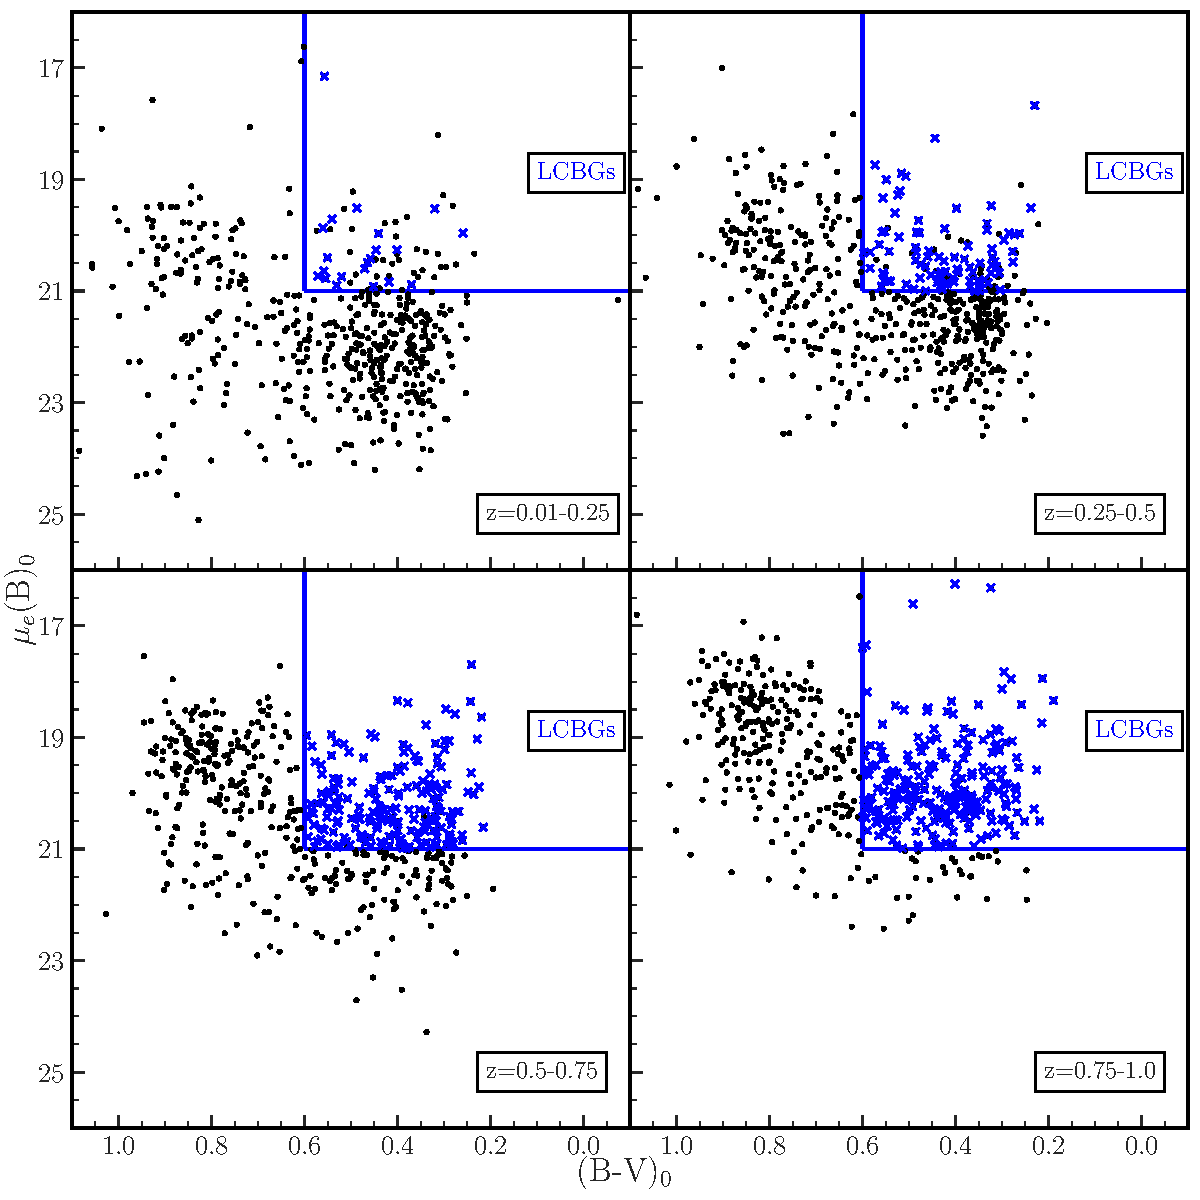
\includegraphics[width=19.05cm]{SurfaceBrightnessColor.pdf}
\caption{Photometric selection criteria for LCBGs. All LCBGs (denoted with a ring around the point) will fall within the shaded region of the B-band surface brightness vs color ($\mu_{e}$(B)$_{0}$ vs (B-V)$_{0}$) plot, but not all points in the shaded region are LCBGs. All values are calculated in the galaxies rest frame. The points are colored to denote whether they fall within the red cloud, green valley, or blue cloud based on their (U-B)$_{0}$ color as characterized by \citet{2006ApJ...647..853W}}
\end{figure*}

\section{Luminosity Function Estimate}
\label{LFE}
\subsection{Luminosity Function Estimator}
The luminosity function is defined as the number of galaxies per comoving volume, per magnitude bin, and is most often characterized using the \citet{1976ApJ...203..297S} parameterization. In magnitudes it is defined as 
\begin{equation}
\phi(M)dM=0.4~ln(10)~\phi^{*}~10^{0.4(M-M^{*})(\alpha+1)}exp(-10^{0.4(M^{*}-M)})dM
\label{eq:equation 6}
\end{equation}
Where $\phi^{*}$ is the characteristic number density of galaxies per unit volume per unit magnitude, M$^{*}$ is the characteristic magnitude where the luminosity function turns over from an exponential into a power law, and $\alpha$ is the characteristic slope of that power law describing the faint end of the luminosity function.
Several methods have been developed to estimate the luminosity function, including \citet{1968ApJ...151..393S,1971MNRAS.155...95L,1979ApJ...231..645T,1979ApJ...234..775T,1986MNRAS.223....1C,1988MNRAS.232..431E}

For our analysis we use the 1/V$_{Max}$ method \citep{1968ApJ...151..393S} which counts galaxies within a known volume. We follow the calculations laid out by \citet{2006ApJ...647..853W} and \citet{2005A&A...439..863I}, described below. The integral luminosity function for a given absolute magnitude is defined as 
\begin{equation}
\int_{M_{bright}}^{M_{faint}}\phi(M)dM=\sum_{i=1}^{N_{G}}\frac{\chi_{i}}{V_{max}(i)}
\label{eq:equation 7}
\end{equation}
where $\chi_{i}$ is the weighting applied to correct for completeness (discussed in Section \ref{sec:Weighting}) and V$_{max}(i)$ is the maximum comoving volume within which a galaxy i with absolute magnitude $M_{i}$ can be detected in the survey,defined as:
\begin{equation}
V_{max}(i)=\int_{\Omega}\int_{z_{min,i}}^{z_{max,i}}\frac{dV}{dz d\Omega}dz d\Omega
\label{eq:equation 8}
\end{equation}
Here, z is redshift, and $\Omega$ is the solid angle of the survey region. In a magnitude limited survey, z$_{min,i}$ and z$_{max,i}$ are defined by:
\begin{equation}
z_{min,i}=min(z_{min},z(M_{i},m_{l}))
\label{eq:equation 9}
\end{equation}
\begin{equation}
z_{max,i}=max(z_{max},z(M_{i},m_{u}))
\label{eq:equation 10}
\end{equation}

where z$_{min}$ and z$_{max}$ are the lower and upper limit of the redshift bin the object occupies, and z(M$_{i}$,m$_{l}$) and z(M$_{i}$,m$_{u}$) are the redshifts at which an object with absolute magnitude M$_{i}$ would no longer fall in the apparent magnitude limits of the survey. We determine the Poisson error using 
\begin{equation}
\sigma_{\phi}=\sqrt{\frac{\chi_{i}}{V_{max,}^{2}(i)}}
\label{eq:equation 11}
\end{equation}

For our calculations we use magnitude bins of 0.5 and redshift bins of 0.2. 
\subsection{Weighting}\label{sec:Weighting}
We must consider galaxies in the survey that have not been directly counted due either to photometric incompleteness or spectroscopic incompleteness. zCOSMOS, the main source of spectroscopic redshifts for our sample, targeted sources with I$_{F814W}$<22.5. We therefore adopt an upper photometric cutoff of m$_{i^{+}}$=22.5 mag and a lower photometric cutoff of m$_{i^{+}}$=15 mag. According to \citet{2017MNRAS.464.1569A}, the photometric catalog is complete to m$_{i^{+}}$=24.5 mag therefore the cutoff we applied requires no photometric correction. We then move to spectroscopic completeness. 

We make two corrections to compensate for spectroscopic incompleteness. The first is correction, for target sampling rate, compensates for the photometrically identified galaxies that have not been targeted in a spectroscopic survey. This weight is defined as:
\begin{equation}
w_{TSR}=\frac{N^{gal}_{Phot}}{N^{gal}_{Spec}}
\label{eq:equation 12}
\end{equation}
where N$^{gal}_{Phot}$ is the number of objects observed in the photometric catalog, and N$^{gal}_{Spec}$ is the number of objects targeted in the spectroscopic survey. We must also correct for objects that were targeted in the spectroscopic survey, but whose redshifts were unable to be definitively determined. This spectroscopic sampling rate weighting is defined as:
\begin{equation}
w_{SSR}=\frac{N^{gal}_{spec}}{N^{gal}_{spec}-N^{fail}_{spec}}
\label{eq:equation 13}
\end{equation}
where N$^{gal}_{spec}$ is the number of galaxies observed spectroscopically, and N$^{fail}_{spec}$ is the number of galaxies where the redshift was indeterminable. If we define the number of galaxies with secure redshifts as N$^{sec}_{spec}$=N$^{gal}_{spec}$-N$^{fail}_{spec}$, then the total weight of each object, $\chi_{i}$, is the multiple of the two weights described above:
\begin{equation}
\chi_{i}=\frac{N^{gal}_{Phot}}{N^{gal}_{Spec}}\frac{N^{gal}_{spec}}{N^{gal}_{spec}-N^{fail}_{spec}}=\frac{N^{gal}_{Phot}}{N^{sec}_{spec}}
\label{eq:equation 14}
\end{equation}
The likelihood of obtaining a secure redshift varies with apparent magnitude, so we calculate weights in magnitude bins of 0.5. Weights range from 1.04 to 5.75 though the high weights only apply to 6 very bright sources with a low target sample rate.
\subsection{Comparison to Previous Work}
\vspace{0.3cm}
\begin{deluxetable*}{rrrrrrrrr}[!htb]
\tablecaption{Fit parameters from our study (1/V$_{max}$) and those in Zucca et al. (2009) (STY)\label{tab:tab1}}
\tablehead{& \multicolumn{4}{l}{This Paper} & \multicolumn{4}{l}{Zucca,2009}\\
\colhead{z-bin} & \colhead{Number} & \colhead{$\alpha_{Vmax}$} & \colhead{M$_{B}^{*}$-5log($h_{70}$)} & \colhead{$\phi^{*}$(10$^{-3}~h^{-3}_{70}~$MPC$^{-3})$} & \colhead{Number} & \colhead{$\alpha_{STY}$} & \colhead{M$_{B}^{*}$-5log($h_{70}$)} & \colhead{$\phi^{*}$(10$^{-3}~h^{-3}_{70}~$MPC$^{-3})$} }
\startdata
$0.1-0.35$&$4039$&$-1.15^{+0.06}_{-0.06}$&$-20.70^{+0.15}_{-0.15}$&$5.85^{+0.93}_{-0.93}$&$1968$&$-1.09^{+0.04}_{-0.04}$&$-20.85^{+0.10}_{-0.11}$&$5.62^{+0.58}_{-0.56}$\\
$0.35-0.55$&$4147$&$-1.03^{+0.06}_{-0.06}$&$-20.69^{+0.07}_{-0.07}$&$6.19^{+0.53}_{-0.53}$&$2059$&$-0.82^{+0.08}_{-0.08}$&$-20.67^{+0.05}_{-0.06}$&$6.40^{+0.58}_{-0.59}$\\
$0.55-0.75$&$3999$&$-0.95^{+0.06}_{-0.06}$&$-20.89^{+0.04}_{-0.04}$&$7.07^{+0.33}_{-0.33}$&$2163$&$-0.85^{+0.11}_{-0.11}$&$-20.98^{+0.09}_{-0.10}$&$6.59^{+0.57}_{-0.61}$\\
$0.75-1.0$&$2993$&$-1.33^{inf}_{inf}$&$-21.12^{inf}_{inf}$&$7.45^{inf}_{inf}$&$1769$&$-1.59^{+0.16}_{-0.16}$&$-21.57^{+0.13}_{-0.15}$&$4.32^{+0.17}_{-0.17}$\\
$0.3-0.8$&$2993$&$-1.10^{+0.06}_{-0.06}$&$-20.89^{+0.08}_{-0.08}$&$5.83^{+0.59}_{-0.59}$&$5249$&$-1.03^{+0.04}_{-0.04}$&$-21.02^{+0.05}_{-0.05}$&$5.42^{+0.32}_{-0.32}$\\
\enddata
\end{deluxetable*}
We are able to directly compare our results with those from \citet{2009A&A...508.1217Z}, who previously studied the effect of environment on the evolution of the luminosity function. Our value for the global luminosity function shows good agreement with theirs in each of their four cited redshift bins between 0.1$\leq$z$\leq$1. Our results are plotted over the Schechter function best fit to their data in figure \ref{fig:LCBGLUMFUNC}. We can also compare Schechter function parameters fit to to our 1/V$_{max}$ calculation with the Schechter function parameters from \citet{2009A&A...508.1217Z} using the STY method. We see in Table \ref{tab:tab1} most fit parameters between the two studies agree within 1-$\sigma$ \todo{I calculated errors using scipy fit package and taking the square root of the }. We do note that our value for the slope of the faint end of the luminosity function does vary at 0.35$\leq$z$\leq$0.55 from that of \citet{2009A&A...508.1217Z} by more than 1-$\sigma$. We also note that the redshift bin 0.75$\leq$z$\leq$1.0 does not sample low luminosity objects, and we are unable to put bounds on our fit to $\alpha$.\todo{Need to play with Magnitude limits or bin sizes to try to generate fit errors}. Comparison with the data from \citet{2009A&A...508.1217Z} seems unreasonable in this bin. Though both studies do have a Schechter Function fit, neither have enough sources dimmer than M$^{*}$ to accurately fit $\alpha$

\section{The LCBG Luminosity Function}\label{sec:Frac}
\begin{deluxetable*}{lrrrrr}[!htb]
\tablecaption{Fit parameters to 1/V$_{max}$ data\label{tab:tab2}}
\tablehead{\colhead{z-bin} & \colhead{Number} & \colhead{$\alpha_{Vmax}$} & \colhead{M$_{B}^{*}$-5log($h_{70}$)} & \colhead{$\phi^{*}$} & \colhead{$j_{B}$}\\ 
 & & & \colhead{(mag)} & \colhead{(10$^{-3}~h^{-3}_{70}~$Mpc$^{-3}$)} & \colhead{(10$^{8}~h_{70}$L$_{\odot}$Mpc$^{-3}$)}}
\startdata
Total Sample\\
$0.01-0.2$&$1253$&$-1.30^{+0.05}_{-0.05}$&$-20.59^{+0.24}_{-0.24}$&$3.46^{+0.77}_{-0.77}$&$1.21^{+0.38}_{-0.38}$\\
$0.2-0.4$&$4573$&$-1.0^{+0.03}_{-0.03}$&$-20.51^{+0.06}_{-0.06}$&$8.87^{+0.56}_{-0.56}$&$2.21^{+0.16}_{-0.16}$\\
$0.4-0.6$&$3171$&$-0.98^{+0.06}_{-0.06}$&$-20.67^{+0.08}_{-0.08}$&$4.85^{+0.42}_{-0.42}$&$1.39^{+0.16}_{-0.16}$\\
$0.6-0.8$&$3888$&$-0.94^{+0.17}_{-0.17}$&$-20.80^{+0.14}_{-0.14}$&$7.39^{+1.05}_{-1.05}$&$2.33^{+0.44}_{-0.44}$\\
$0.8-1.0$&$2507$&$-0.85^{+0.15}_{-0.15}$&$-20.905^{+0.08}_{-0.08}$&$8.93^{+0.56}_{-0.56}$&$2.99^{+0.28}_{-0.28}$\\
$0.3-0.8$&$10077$&$-1.053^{+0.08}_{-0.08}$&$-20.852^{+0.10}_{-0.10}$&$5.83^{+0.67}_{-0.67}$&$2.05^{+0.31}_{-0.31}$\\
\tableline
LCBGs\\
$0.01-0.2$&$27$&$-0.61^{+0.37}_{-0.37}$&$-20.33^{+0.41}_{-0.41}$&$0.71^{+0.27}_{-0.27}$&$0.13^{+0.07}_{-0.07}$\\
$0.2-0.4$&$508$&$-1.06^{+0.24}_{-0.24}$&$-20.08^{+0.25}_{-0.25}$&$1.51^{+0.45}_{-0.45}$&$0.29^{+0.07}_{-0.07}$\\
$0.4-0.6$&$838$&$-0.86^{+0.14}_{-0.14}$&$-20.55^{+0.17}_{-0.17}$&$1.53^{+0.27}_{-0.27}$&$0.37^{+0.09}_{-0.09}$\\
$0.6-0.8$&$1342$&$-0.88^{+0.36}_{-0.36}$&$-20.56^{+0.26}_{-0.26}$&$3.24^{+0.81}_{-0.81}$&$0.77^{+0.28}_{-0.28}$\\
$0.8-1.0$&$1131$&$-1.12^{+0.21}_{-0.21}$&$-20.86^{+0.12}_{-0.12}$&$4.30^{+0.49}_{-0.49}$&$1.61^{+0.25}_{-0.25}$\\
$0.3-0.8$&$2571$&$-0.52^{+0.15}_{-0.15}$&$-20.37^{+0.13}_{-0.13}$&$2.68^{+0.28}_{-0.28}$&$0.52^{+0.08}_{-0.08}$\\
\enddata
\end{deluxetable*}
\begin{center}
\begin{figure*}
\includegraphics[width=20cm]{LUMFUNCPLOTS.pdf}
\caption{Luminosity function for the entire galaxy population (green) and LCBGs (blue). Points marked with an x are not considered in our fit. They are most often regions of M$_{B}$-z space that are not sampled well enough to give a proper estimate of $\Phi$ in that bin. The histogram below each plot shows the log$_{10}$ of the number of objects in each bin, with the white bars being total galaxies, and the gray bars being LCBGs. The number in each bin is listed above each bar. }
\label{fig:LCBGLUMFUNC}
\end{figure*}
\end{center}
The fit parameters in redshift bins of z=0.2 are shown in Table \ref{tab:tab2}. We are covering approximately the same redshift range as above, and we see a similar trend in the evolution of M$^{*}$, approximately 0.5 between 0$\leq$z$\leq$1. The evolution of M$^{*}$ in the LCBG population is greater, evolving by roughly 0.7 over the same redshift range. This should be expected as both \citet{2006ApJ...647..853W} and \citet{2015ApJ...815...94B} have found stronger evolution of M$^{*}$ in blue galaxies than red over the same range. This evolution is consistent with cosmic downsizing \citet{1996AJ....112..839C} of the blue population of galaxies, wherein the brighter galaxies exhaust their ability to form stars and fade, leaving smaller, less luminous blue galaxies in the local universe.
Evolution of M$^{*}$ and $\phi^{*}$ can be seen in Figures \ref{fig:EVMSTAR} and \ref{fig:EVPHISTAR}. 
\begin{center}
\begin{figure}
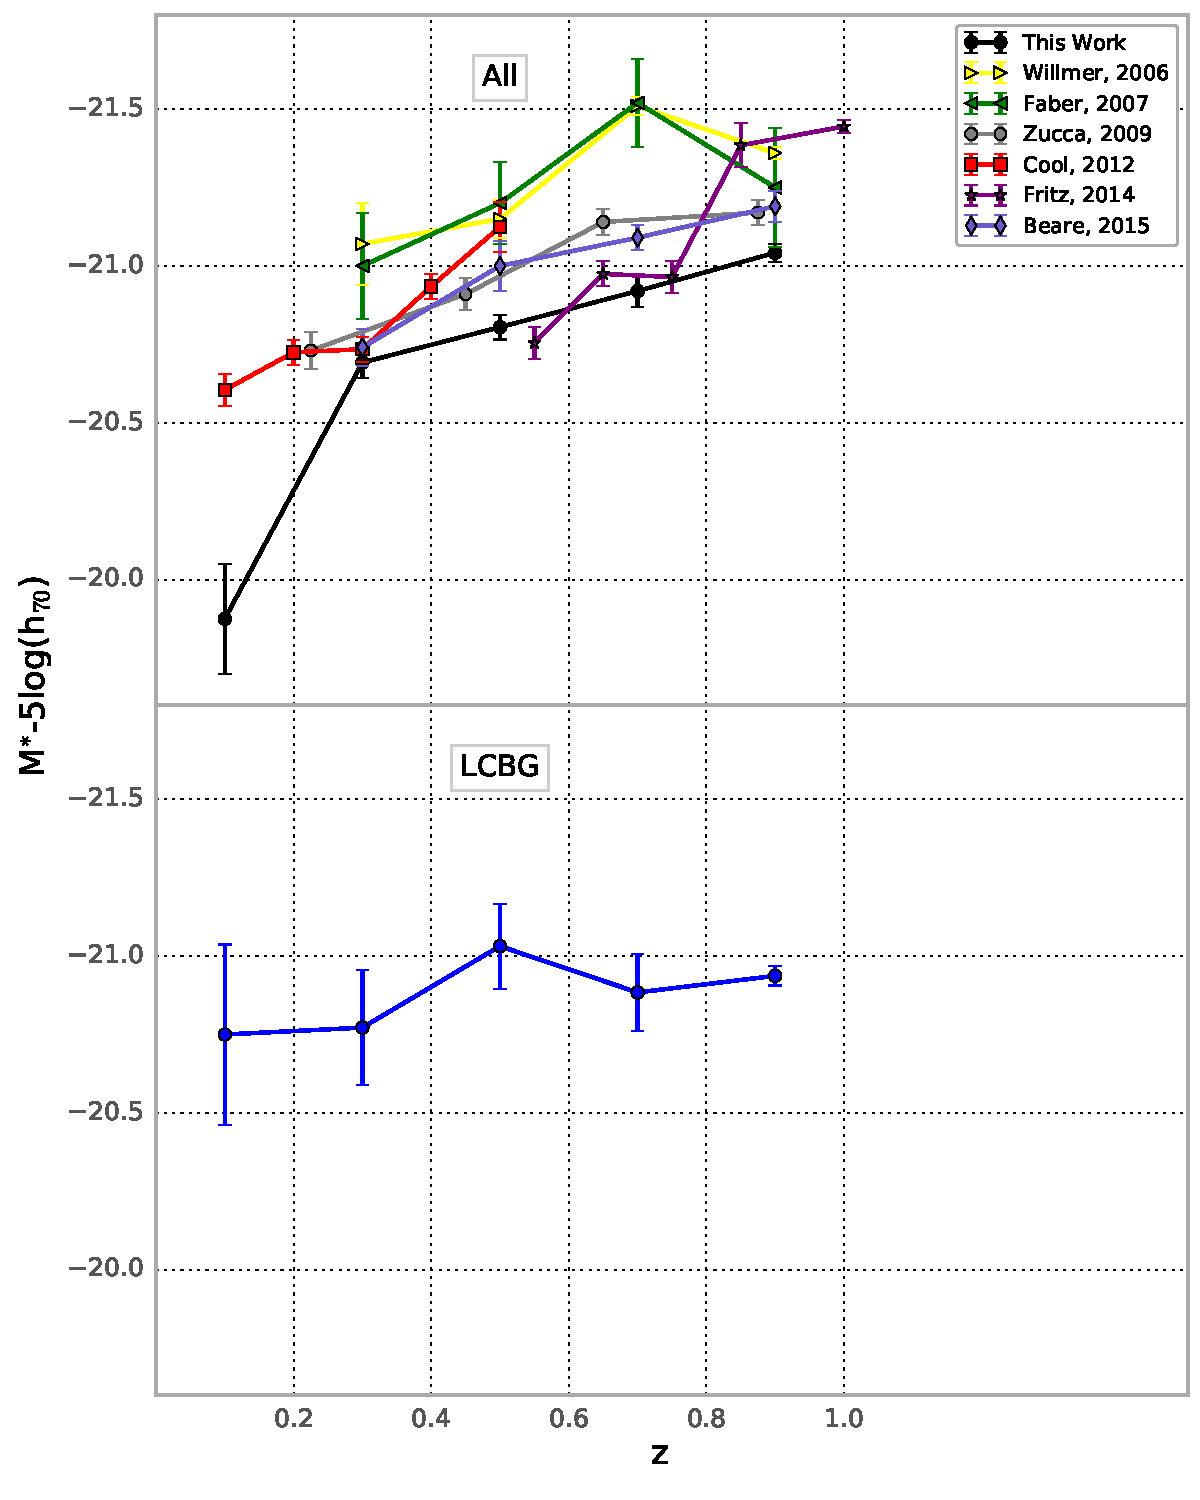
\includegraphics{EVMSTAR.pdf}
\caption{Evolution of M$^{*}$ with redshift}
\label{fig:EVMSTAR}
\end{figure}
\end{center}
\begin{center}
\begin{figure}
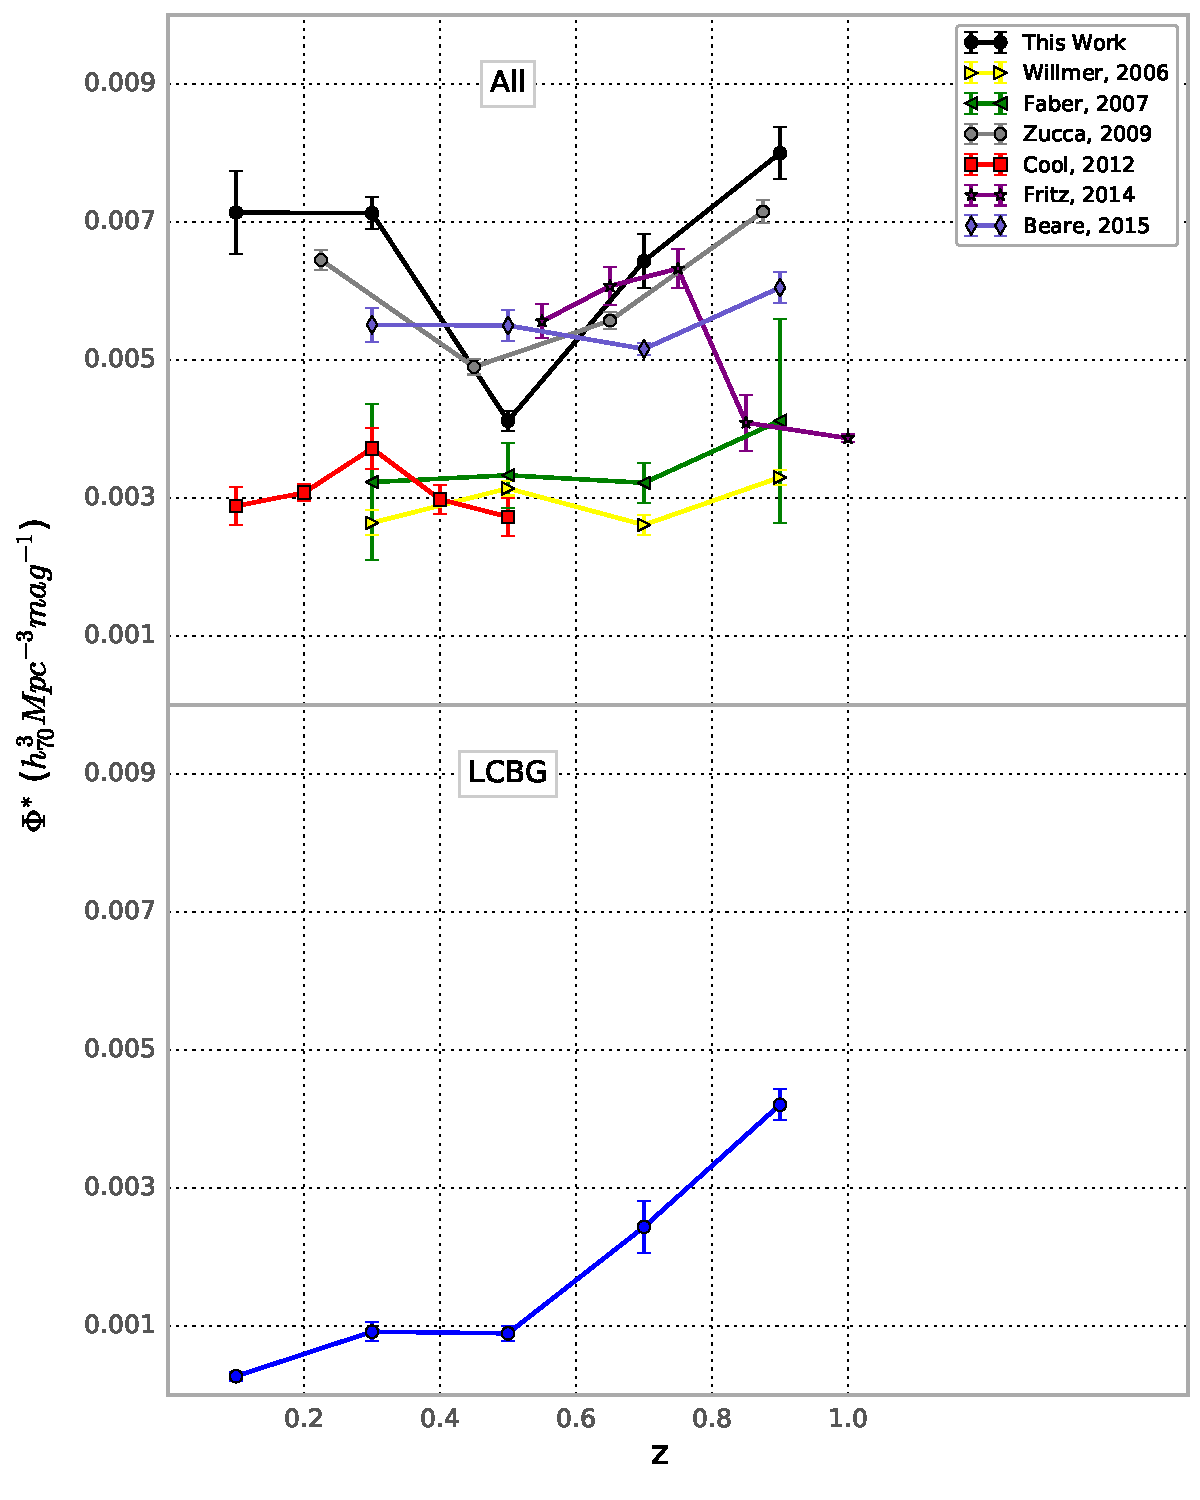
\includegraphics{EVPHISTAR.pdf}
\caption{Evolution of $\phi^{*}$ with redshift}
\label{fig:EVPHISTAR}
\end{figure}
\end{center}

As discussed in section 8.4 of \citet{2015ApJ...815...94B}, previous literature agrees that $\phi^{*}$ and M$^{*}$ evolve for most galaxy populations, but there is little agreement in how much they vary. This can be attributed to the degenerate 60nature of the Schechter parameters, and in particular the variance in $\phi^{*}$ and M$^{*}$ with the adopted value of $\alpha$. Measurements of the luminosity density vary much less than those of the Schechter parameters because it depends on both $\phi^{*}$ and M$^{*}$. The luminosity density is calculated as:
\begin{equation}
j=\phi^{*}L^{*}\Gamma(\alpha+2)
\end{equation}
where $L^{*}$ is the characteristic luminosity calculated from the characteristic magnitude. We have plotted luminosity density ($j_{B}$) in Figure \ref{fig:LUMDENSEV}. We have not used a consistent $\alpha$ to derive numbers for $j$ but we do see that it evolves similarly to figure 16 from \citet{2015ApJ...815...94B}. The evolution of $j_{B}$ for the total population in both samples is entirely consistent, while the evolution in LCBGs roughly matches the \citet{2015ApJ...815...94B} blue population at high redshift, but seems to show more evolution over the redshift range 0$\leq$z$\leq$1.

We integrate the LCBG luminosity function from M=-$\infty$ to -18.5 to estimate the evolution of LCBG density between 0$\leq$z$\leq$1. At the highest redshift range in our sample, 0.8$\leq$z$\leq$1, the LCBG density is 8.3$\times$10$^{-3}h_{70}^{3}$Mpc$^{-3}$ and at the lowest, 0.01$\leq$z$\leq$0.2, it is 7.2$\times$10$^{-4}h_{70}^{3}$Mpc$^{-3}$. This is an order of magnitude fall-off between 0$\leq$z$\leq$1, consistent with what was suggested in \citet{2004ApJ...617.1004W}. We have plotted the number density of LCBGs with redshift in Figure \ref{fig:NumDensEv} to more clearly show the evolution. This shows the consistency with \citet{2004ApJ...617.1004W}, and with \citet{1997ApJ...489..543P} quite clearly. You can see that between 0.5$\leq$z$\leq$1, the number density rapidly drops by about a factor of four and then slowly decreases by about a factor of two between 0$\leq$z$\leq$0.5. 

\begin{center}
\begin{figure}
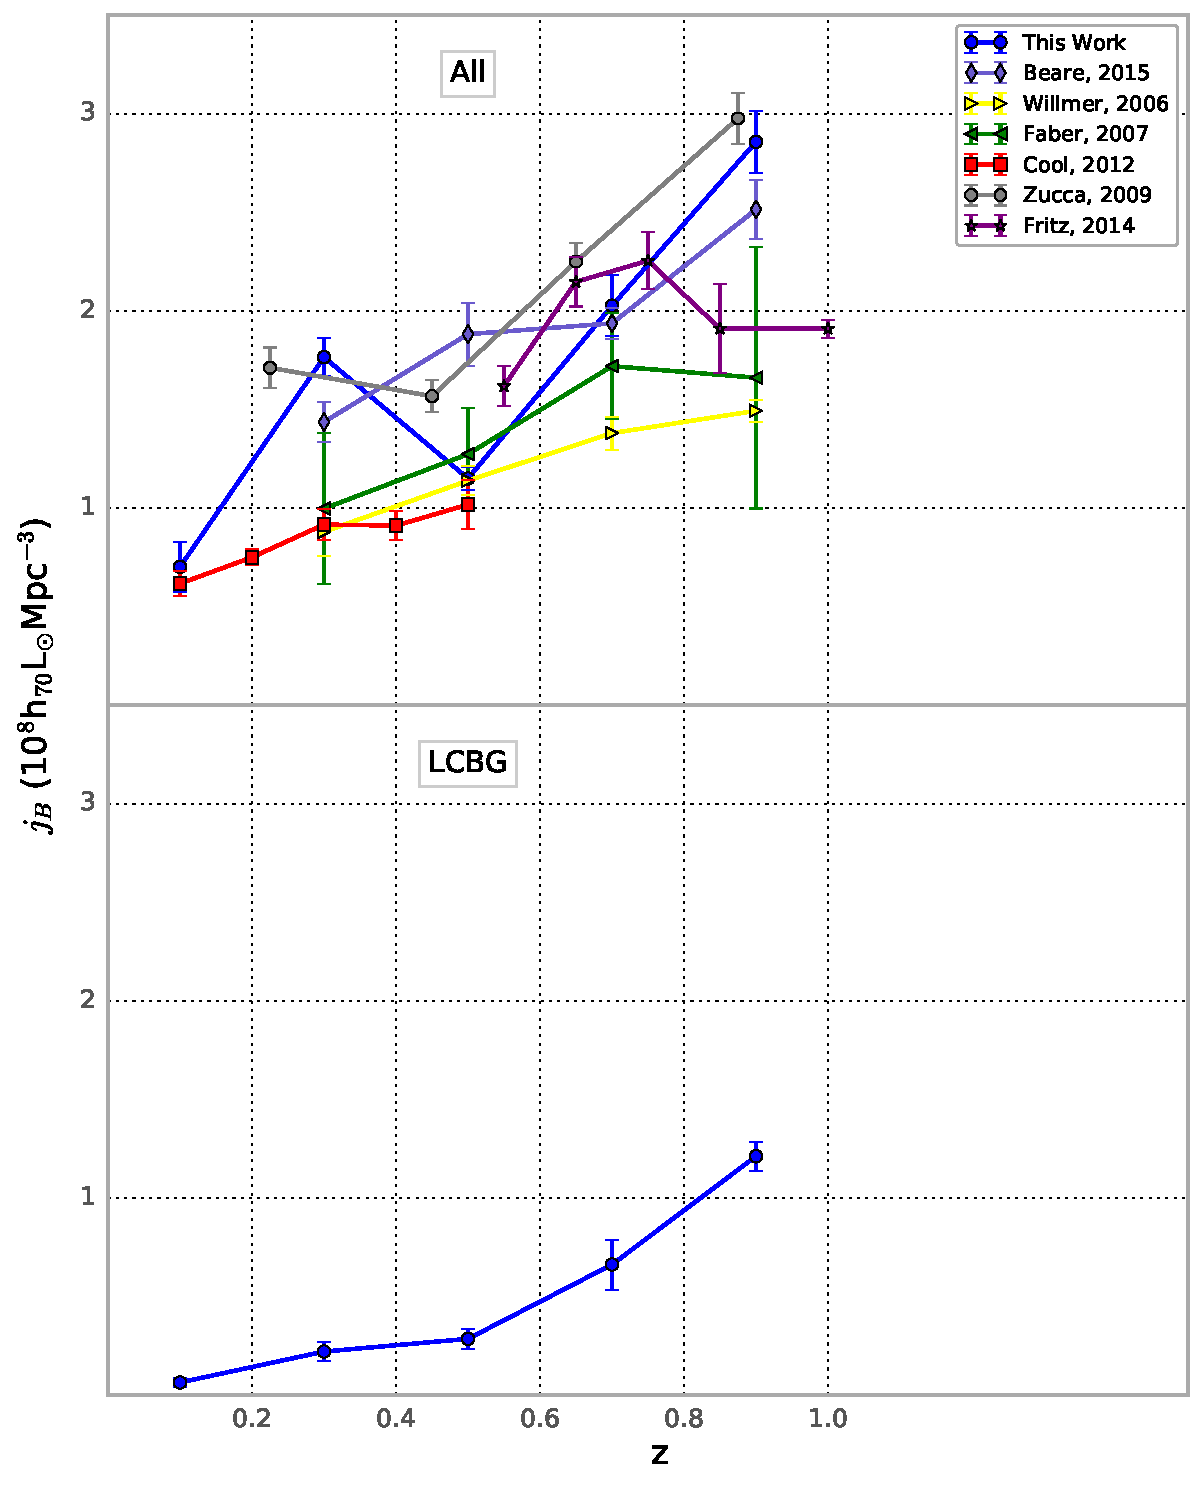
\includegraphics[width=14cm]{LUMDENSEV.pdf}
\caption{Evolution of $j_{B}$ with redshift}
\label{fig:LUMDENSEV}
\end{figure}
\end{center}


To directly compare our method with \citet{1997ApJ...489..543P} we have generated the LCBG luminosity function in the redshift ranges 0.7$\leq$z$\leq$1 and 0.4$\leq$z$\leq$0.7 and calculated the number density. As per \citet{2004ApJ...617.1004W}, we use the absolute magnitude cut-off from \citet{1997ApJ...489..543P}, M=$-20-5log_{10}(h_{50})$ or M=-19.27, as our luminosity cut-off at z=0.85 and the LCBG absolute magnitude cut-off of M=-18.5 at z=0.55. We find at z=0.85 the LCBG number density is 4.0$\times$10$^{-3}h_{70}^{3}$Mpc$^{-3}$ compared to the value from \citet{1997ApJ...489..543P} of 3.3$\times$10$^{-3}h_{70}^{3}$Mpc$^{-3}$. At z=0.55 we find the LCBG number density to be 2.7$\times$10$^{-3}h_{70}^{3}$Mpc$^{-3}$ compared to the value from \citet{1997ApJ...489..543P} of 1.8$\times$10$^{-3}h_{70}^{3}$Mpc$^{-3}$. 

\begin{center}
\begin{figure}
\includegraphics[width=20cm]{NumberDensity.pdf}
\caption{Number density of LCBGs in the COSMOS field. Also plotted are the points from \citet{1997ApJ...489..543P}, and \citet{2004ApJ...617.1004W}}
\label{fig:NumDensEv}
\end{figure}
\end{center}

We can also look at LCBGs as a fraction of the total population. This is done in three ways, all plotted in Figure \ref{fig:Fracev}. Plot a shows all LCBGs divided by all galaxies in the G10/COSMOS region . Plot b shows the number density of LCBGs divided by the number density of all galaxies brighter than -18.5 calculated by integrating the luminosity function. Plot c shows the number density of LCBGs divided by the number density of galaxies brighter than -15. We can see the fraction of LCBGs between 0$\leq$z$\leq$1 in plot a and c match well. This makes sense, as galaxies with M$_{B}$=-15 are only detectable in the lower redshift bin of the COSMOS survey. The middle redshift bins in plots a and b match relatively well, and this too can be explained roughly because the G10/COSMOS source catalog still contains sources around M$_{B}$=-18.5. The final redshift bin in plot a, showing the fraction of LCBGs in COSMOS, is limited by the photometry to sources brighter than -20.5. Therefore, the fraction should not match plot b, LCBGs as a fraction of galaxies brighter than M$_{B}$=-18.5, nor plot c, LCBGs as a fraction of galaxies brighter than M$_{B}$=-15.

\begin{center}
\begin{figure}[!ht]
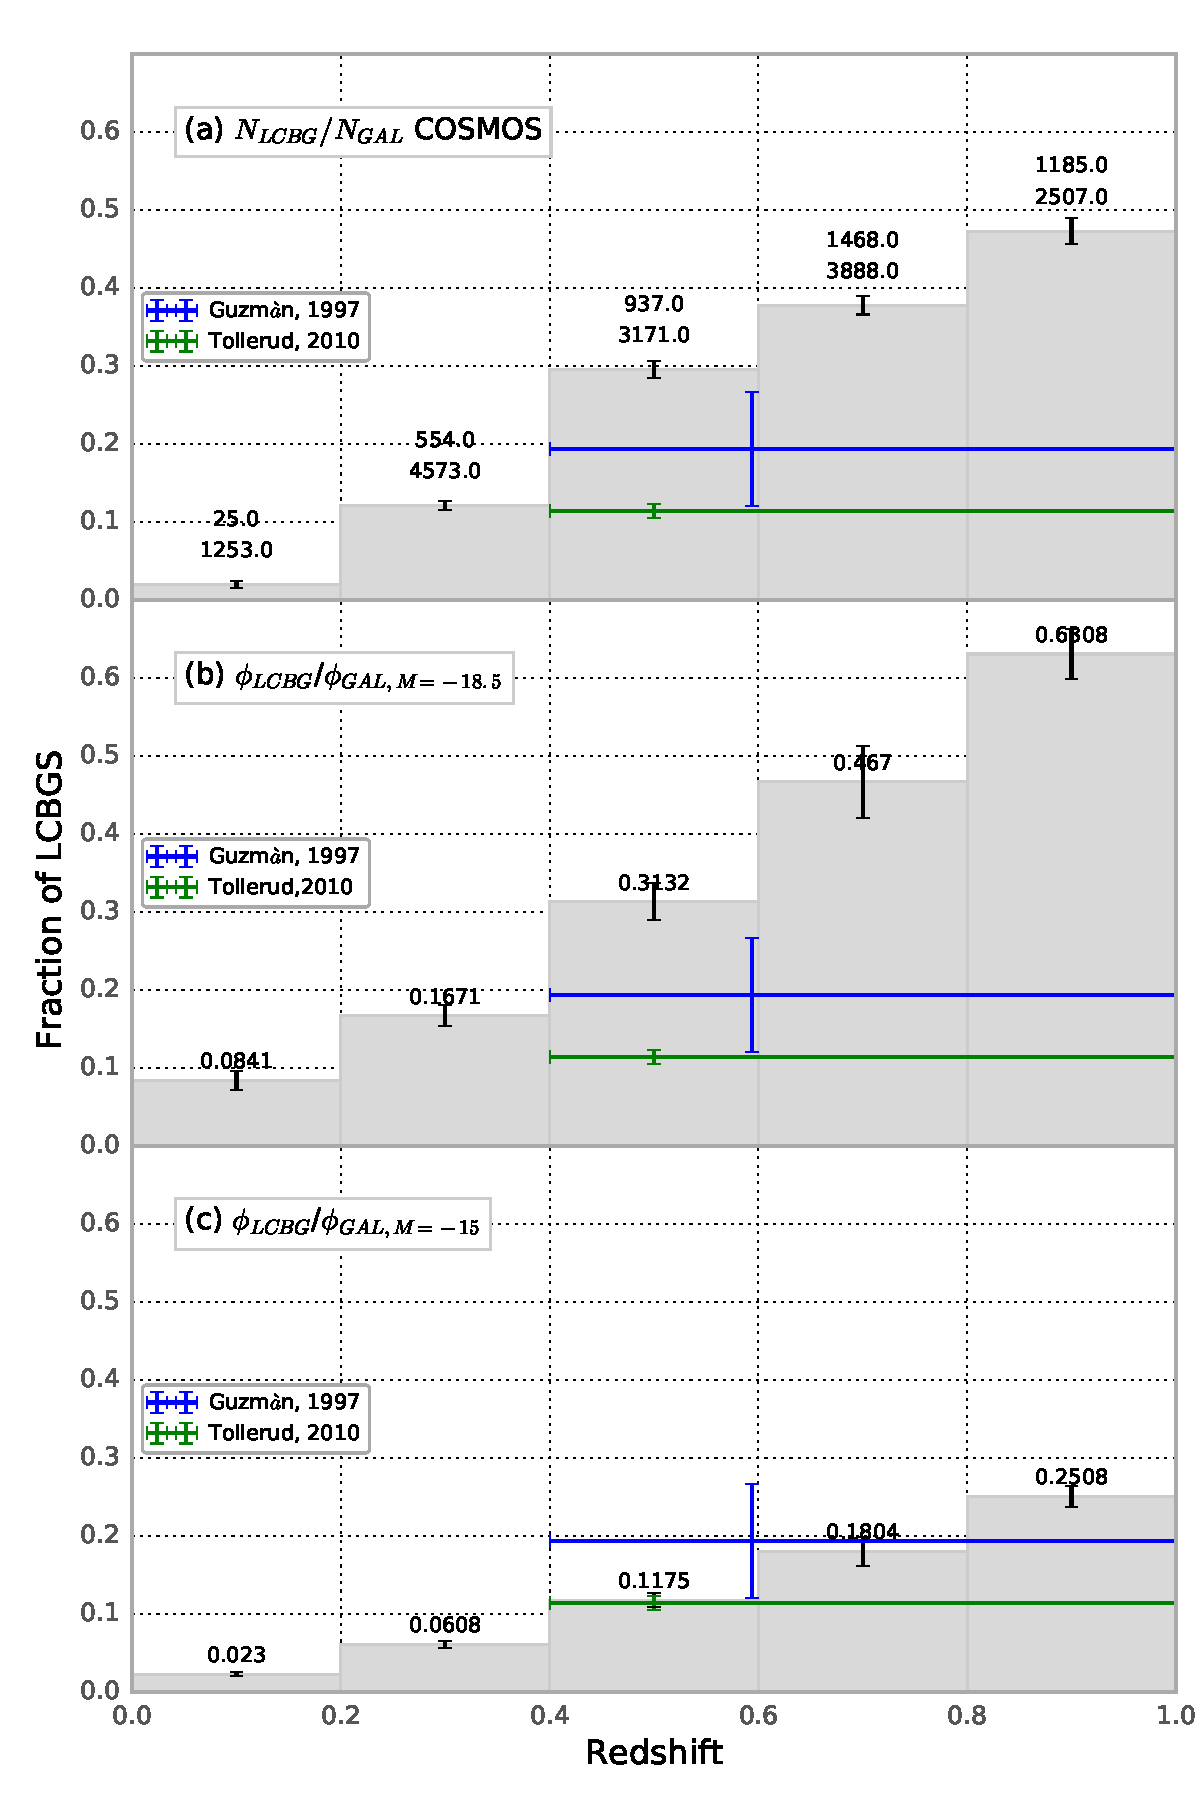
\includegraphics[width=13cm]{FractionLCBGPLOT.pdf}
\caption{Evolution of the fraction of LCBGs in (a) COSMOS (b) integrating both the total sample luminosity function and the LCBG luminosity function to M$_{B}$=-18.5 and (c) integrating the total sample luminosity function to M$_{B}$=-15. We have also included values from the literature }
\label{fig:Fracev}
\end{figure}
\end{center}

\section{Conclusion}\label{sec:Conc}
We have used data from the G10/COSMOS survey region to trace the evolution of the LCBG population between 0$\leq$z$\leq$1. We have done this by generating the luminosity function of the total galaxy population and of LCBGs in redshift intervals of z=0.2. We have found that the LCBG population appears to evolve rapidly as previously suggested, with the number density at z=0.9 approximately an order of magnitude larger than that at z=0.1. 

We see evolution of $\sim$0.8 in M$^{*}$ and $\sim$6 in $\phi^{*}$ both increasing from z=0.1 to z=0.9. Knowing that Schechter parameters are degenerate, and in particular M$^{*}$ and $\phi^{*}$ are dependent on the value of $\alpha$, we also looked at the evolution of the less degenerate luminosity density. We find that it increases  by a factor of 12 betweeon z=0.1 and z=0.9. Finally, we can see that LCBGs make up a significant fraction of all galaxies at z=0.9. They make up approximately 30\% of the galaxy population brighter than M=-15. In the same vein, we see that they make up less than 2\% of galaxies in the nearby universe. \todo{needs more}  The rapid change in number density and luminosity density are both consistent with LCBGs being the most rapidly evolving galaxy population between 0$\leq$z$\leq$1.

We can use this large statistical sample of LCBGs to learn how they are effected by environment. Information from \citet{2012ApJ...755...48K} shows which galaxies in the COSMOS sample are isolated, in groups, and in clusters. We can combine this with the G10/COSMOS data to determine various photometric properties of LCBGs in different environments and also search for change of preferred environment with redshift for example. 




\acknowledgments
Acknowledgments.

%\facility{facility ID}
\facilities{facility ID, facility ID, facility ID} 
\software{Numpy}
\bibstyle{plain}
\bibliography{lcbg_lf}
%\begin{thebibliography}{99}
%\bibitem[Ahn et al.(2014)]{2014ApJS..211...17A} Ahn, C.~P., Alexandroff, R., Allende Prieto, C., et al.\ 2014, \apjs, 211, 17 
%\bibitem[Andrews et al.(2017)]{2017MNRAS.464.1569A} Andrews, S.~K., Driver, S.~P., Davies, L.~J.~M., et al.\ 2017, \mnras, 464, 1569
%\bibitem[Baldry et al.(2014)]{2014MNRAS.441.2440B} Baldry, I.~K., Alpaslan, M., Bauer, A.~E., et al.\ 2014, \mnras, 441, 2440 
%\bibitem[Blanton \& Roweis(2007)]{2007AJ....133..734B} Blanton, M.~R., \& Roweis, S.\ 2007, \aj, 133, 734
%\bibitem[Beare et al.(2015)]{2015ApJ...815...94B} Beare, R., Brown, M.~J.~I., Pimbblet, K., Bian, F., \& Lin, Y.-T.\ 2015, \apj, 815, 94 
%\bibitem[Capak et al.(2007)]{2007ApJS..172...99C} Capak, P., Aussel, H., Ajiki, M., et al.\ 2007, \apjs, 172, 99
%\bibitem[Coil et al.(2011)]{2011ApJ...741....8C} Coil, A.~L., Blanton, M.~R., Burles, S.~M., et al.\ 2011, \apj, 741, 8 
%\bibitem[Cool et al.(2013)]{2013ApJ...767..118C} Cool, R.~J., Moustakas, J., Blanton, M.~R., et al.\ 2013, \apj, 767, 118
%\bibitem[Cowie et al.(1996)]{1996AJ....112..839C} Cowie, L.~L., Songaila, A., Hu, E.~M., \& Cohen, J.~G.\ 1996, \aj, 112, 839 
%\bibitem[Davies et al.(2015)]{2015MNRAS.447.1014D} Davies, L.~J.~M., Driver, S.~P., Robotham, A.~S.~G., et al.\ 2015, \mnras, 447, 1014
%\bibitem[Garilli et al.(2008)]{2008A&A...486..683G} Garilli, B., Le F{\`e}vre, O., Guzzo, L., et al.\ 2008, \aap, 486, 683 
%\bibitem[Garland et al.(2004)]{2004ApJ...615..689G} Garland, C.~A., Pisano, D.~J., Williams, J.~P., Guzm{\'a}n, R., \& Castander, F.~J.\ 2004, \apj, 615, 689 
%\bibitem[Ilbert et al.(2005)]{2005A&A...439..863I} Ilbert, O., Tresse, L., Zucca, E., et al.\ 2005, \aap, 439, 863 
%\bibitem[Ilbert et al.(2009)]{2009ApJ...690.1236I} Ilbert, O., Capak, P., Salvato, M., et al.\ 2009, \apj, 690, 1236 
%\bibitem[Koekemoer et al.(2007)]{2007ApJS..172..196K} Koekemoer, A.~M., Aussel, H., Calzetti, D., et al.\ 2007, \apjs, 172, 196
%\bibitem[Lange et al.(2015)]{2015MNRAS.447.2603L} Lange, R., Driver, S.~P., Robotham, A.~S.~G., et al.\ 2015, \mnras, 447, 2603 
%\bibitem[Lilly et al.(2009)]{2009ApJS..184..218L} Lilly, S.~J., Le Brun, V., Maier, C., et al.\ 2009, \apjs, 184, 218 
%\bibitem[McCracken et al.(2012)]{2012A&A...544A.156M} McCracken, H.~J., Milvang-Jensen, B., Dunlop, J., et al.\ 2012, \aap, 544, A156
%\bibitem[Oliver et al.(2012)]{2012MNRAS.424.1614O} Oliver, S.~J., Bock, J., Altieri, B., et al.\ 2012, \mnras, 424, 1614
%\bibitem[P{\'e}rez-Gallego et al.(2011)]{2011MNRAS.418.2350P} P{\'e}rez-Gallego, J., Guzm{\'a}n, R., Castillo-Morales, A., et al.\ 2011, \mnras, 418, 2350 
%\bibitem[Sanders et al.(2007)]{2007ApJS..172...86S} Sanders, D.~B., Salvato, M., Aussel, H., et al.\ 2007, \apjs, 172, 86 
%\bibitem[Schechter(1976)]{1976ApJ...203..297S} Schechter, P.\ 1976, \apj, 203, 297 
%\bibitem[Schmidt(1968)]{1968ApJ...151..393S} Schmidt, M.\ 1968, \apj, 151, 393
%\bibitem[Scoville et al.(2007)]{2007ApJS..172....1S} Scoville, N., Aussel, H., Brusa, M., et al.\ 2007, \apjs, 172, 1
%\bibitem[Taniguchi et al.(2007)]{2007ApJS..172....9T} Taniguchi, Y., Scoville, N., Murayama, T., et al.\ 2007, \apjs, 172, 9
%\bibitem[Taniguchi et al.(2015)]{2015PASJ...67..104T} Taniguchi, Y., Kajisawa, M., Kobayashi, M.~A.~R., et al.\ 2015, \pasj, 67, 104 
%\bibitem[Tasca et al.(2009)]{2009A&A...503..379T} Tasca, L.~A.~M., Kneib, J.-P., Iovino, A., et al.\ 2009, \aap, 503, 379 
%\bibitem[Werk et al.(2004)]{2004ApJ...617.1004W} Werk, J.~K., Jangren, A., \& Salzer, J.~J.\ 2004, \apj, 617, 1004 
%\bibitem[Willmer et al.(2006)]{2006ApJ...647..853W} Willmer, C.~N.~A., Faber, S.~M., Koo, D.~C., et al.\ 2006, \apj, 647, 853 
%\bibitem[Wright et al.(2016)]{2016MNRAS.460..765W} Wright, A.~H., Robotham, A.~S.~G., Bourne, N., et al.\ 2016, \mnras, 460, 765 
%\bibitem[Zamojski et al.(2007)]{2007ApJS..172..468Z} Zamojski, M.~A., Schiminovich, D., Rich, R.~M., et al.\ 2007, \apjs, 172, 468 
%\bibitem[Zucca et al.(2009)]{2009A&A...508.1217Z} Zucca, E., Bardelli, S., Bolzonella, M., et al.\ 2009, \aap, 508, 1217 
%\end{thebibliography}
\appendix
\section{appendix section}

\end{document}